% Adjusting chapter title format for regular (numbered) chapters
\titleformat{\chapter}[display]
  {\normalfont\huge\bfseries\centering}{\chaptertitlename\ \thechapter}{20pt}{\Huge}

% Using similar styling for unnumbered chapters but without "Chapter" prefix
\titleformat{name=\chapter,numberless}
  {\normalfont\huge\bfseries\centering}{}{0pt}{\Huge}

\titlespacing*{\chapter}{0pt}{50pt}{40pt} % Adjust vertical spacing before and after the title

\definecolor{barblue}{RGB}{153,204,254}
\definecolor{groupblue}{RGB}{51,102,254}
\definecolor{linkred}{RGB}{165,0,33}
\chapter{PhD Two-Year Plan} % Ensures chapter numbering starts correctly
\label{chp:9}

\section{Research Modules}
I have categorized my research into seven modules as depicted in Figure \ref{fig:no_publish}: Module 1 (DNN Testing Framework), Module 2 (Specification), Module 3 (Sampling), Module 4 (Interpretability), Module 5 (Testcase Generation), Module 6 (Coverage Criteria), and Module 7 (Error Summarization).

\begin{figure}[ht]
  \centering
  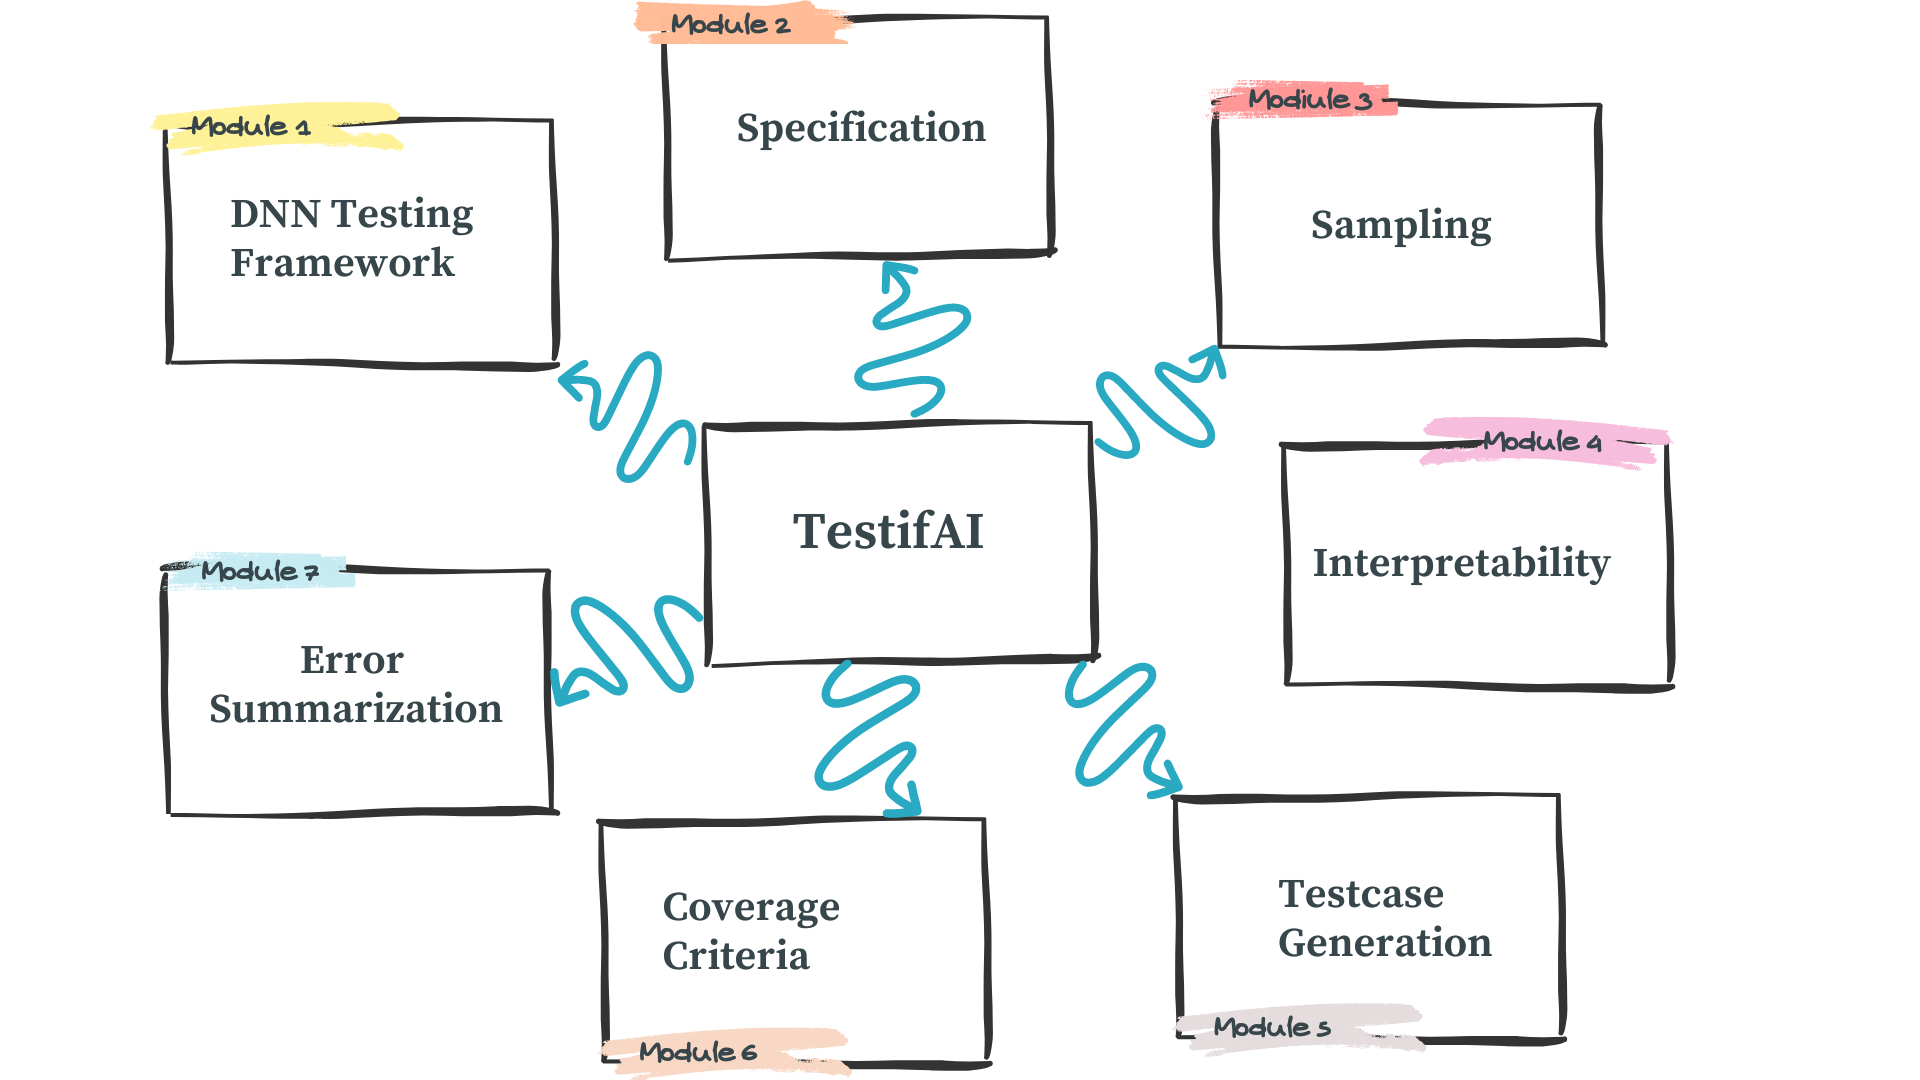
\includegraphics[width=\linewidth]{researchareas.png}
  \caption{Research Modules}
  \label{fig:no_publish}
\end{figure}

\section{Mapping of Research Modules to Objectives}
The research is structured into seven distinct modules, each addressing a specific objective. Table \ref{table:modules} outlines the mapping of these research modules to their corresponding objectives discussed in Section \ref{sec:research_objectives}.

\begin{table}[ht]
  \centering
  \renewcommand{\arraystretch}{1.5} % Adjusts the row padding
  \begin{tabular}{|l|l|}
    \hline
    \rowcolor[HTML]{000000} 
    \multicolumn{1}{|c|}{\cellcolor[HTML]{000000}{\color[HTML]{FFFFFF} \textbf{Research Modules}}} & {\color[HTML]{FFFFFF} \textbf{Research Objectives}} \\ \hline
    {\color[HTML]{404040} DNN Testing Framework} & Obj1 \\ \hline
    {\color[HTML]{404040} Specification} & Obj2 \\ \hline
    {\color[HTML]{404040} Sampling} & Obj3 \\ \hline
    {\color[HTML]{404040} Interpretability} & Obj4 \\ \hline
    {\color[HTML]{404040} Testcase Generation} & Obj5 \\ \hline
    {\color[HTML]{404040} Coverage Criteria} & Obj6 \\ \hline
    Error Summarization & Obj7 \\ \hline
  \end{tabular}
  \caption{Mapping of Research Modules to Objectives}
  \label{table:modules}
\end{table}

These modules are further divided into specific tasks to streamline the research process:

\subsection{DNN Testing Framework (Module 1, 43\% completion)}
\subsubsection{Literature review (M\textsubscript{1} - M\textsubscript{5}, 60\% completion)}
Outline comprehensive testing requirements.

\subsubsection{Designing a conceptual framework (M\textsubscript{8} - M\textsubscript{12}, 100\% completion)}
Set clear criteria for evaluating test outcomes.

\subsubsection{Design local and global coverage flow (M\textsubscript{8} - M\textsubscript{10}, 70\% completion)}
Set clear criteria for evaluating test outcomes.

\subsubsection{Implementing the Simple real life Example to cauclate local to global robustness(M\textsubscript{8} - M\textsubscript{10}, 100\% completion)}
Implement Adder for this

\subsubsection{Implementing ProbLog for  calculating global robustness with one example (M\textsubscript{9} - M\textsubscript{11}, 100\% completion)}
Set clear criteria for evaluating test outcomes.

\subsubsection{Integrate ProbLog code with python code (M\textsubscript{9} - M\textsubscript{11}, 100\% completion)}
Set clear criteria for evaluating test outcomes.

\subsubsection{Integrate interpratability analysis to identify critical features (M\textsubscript{Oct24} - M\textsubscript{Dec24}, 0\% completion)}
Set clear criteria for evaluating test outcomes.
\subsubsection{Integrate efficient sampling approach (M\textsubscript{Jan25} - M\textsubscript{Feb25}, 0\% completion)}
Set clear criteria for evaluating test outcomes.

\subsubsection{Integrate error summarzation modules(M\textsubscript{March25} - M\textsubscript{May25}, 0\% completion)}
Set clear criteria for evaluating test outcomes.
\subsubsection{Integrate all developed techniques (M\textsubscript{Sep25} - M\textsubscript{Oct25}, 0\% completion)}
Set clear criteria for evaluating test outcomes.
\subsubsection{Generate results on different datasets  and make scenarios to validate this framework (M\textsubscript{Sep25} - M\textsubscript{Oct25}, 0\% completion)}
Set clear criteria for evaluating test outcomes.





\subsection{Specification (Module 2, 0\% completion)}
\subsubsection{Find a way to define specification, how to  formalize it (M\textsubscript{20} - M\textsubscript{23}, 0\% completion)}
Outline comprehensive testing requirements.

\subsubsection{How to pass specifications to ProbLog (M\textsubscript{20} - M\textsubscript{23}, 0\% completion)}
Set clear criteria for evaluating test outcomes.

\subsubsection{How to automatically change specifications into desired format of framework(M\textsubscript{20} - M\textsubscript{23}, 0\% completion)}
Set clear criteria for evaluating test outcomes.



\subsection{Sampling (Module 3, 45\% completion)}
\subsubsection{Reading Papers Related to Sampling Techniques and Identify Gaps (M\textsubscript{9} - M\textsubscript{10}, 50\% completion)}
M\textsubscript{9} - M\textsubscript{10}, 50\% completion.

\subsubsection{Develop Efficient Sampling Technique (M\textsubscript{10} - M\textsubscript{12}, 0\% completion))}
Develop a technique that will cover all inputs or corner cases (M\textsubscript{10} - M\textsubscript{12}, 0\% completion).

\subsubsection{Implement Existing Sampling Techniques (M\textsubscript{9} - M\textsubscript{10}, 30\% completion)}
Identify corner cases and prioritize those corner cases (M\textsubscript{9} - M\textsubscript{10}, 30\% completion).

\subsubsection{Automate sample generation according to specification(M\textsubscript{9} - M\textsubscript{10}, 0\% completion)}
M\textsubscript{9} - M\textsubscript{10}, 0\% completion.

\subsection{Interpretability (Module 4, 42\% completion)}
\subsubsection{Literature Review (M\textsubscript{4} - M\textsubscript{24}, 30\% completion)}
M\textsubscript{4} - M\textsubscript{24}, 30\% completion.

\subsubsection{Implementation of SHAP Tool (M\textsubscript{4} - M\textsubscript{6}, 80\% completion)}
M\textsubscript{4} - M\textsubscript{6}, 80\% completion.

\subsubsection{Applying SHAP to Identify Important Pixels (M\textsubscript{4} - M\textsubscript{5}, 80\% completion)}
M\textsubscript{4} - M\textsubscript{5}, 80\% completion.

\subsubsection{Explore Other Interpretability Analysis Techniques (M\textsubscript{15} - M\textsubscript{17}, 0\% completion)}
Explore techniques such as LIME to identify key features that can guide the generation of optimal test cases for evaluating model robustness (M\textsubscript{15} - M\textsubscript{17}, 0\% completion).

\subsubsection{Automate Interpretability Approach in Test Case Generation Module (M\textsubscript{16} - M\textsubscript{17}, 0\% completion)}
M\textsubscript{16} - M\textsubscript{17}, 0\% completion.

\subsection{Testcase Generation (Module 5, 50\% completion)}
\subsubsection{Literature Review (M\textsubscript{1} - M\textsubscript{18}, 50\% completion)}
M\textsubscript{1} - M\textsubscript{18}, 50\% completion.

\subsubsection{Exploring Libraries for Test Case Generation (M\textsubscript{1} - M\textsubscript{2}, 80\% completion)}
M\textsubscript{1} - M\textsubscript{2}, 80\% completion.

\subsubsection{Implementing Adversarial Attacks and Semantic Adversarial Test Cases (M\textsubscript{3} - M\textsubscript{4}, 80\% completion)}
M\textsubscript{3} - M\textsubscript{4}, 80\% completion.

\subsubsection{Apply Existing Test Case Generation Methods to Benchmark Datasets (Analyze the results (M\textsubscript{13} - M\textsubscript{14}, 0\% completion))}
Analyze the results (M\textsubscript{13} - M\textsubscript{14}, 0\% completion).

\subsubsection{Automate Proposed Test Generation Module (M\textsubscript{15} - M\textsubscript{16}, 0\% completion)}
M\textsubscript{15} - M\textsubscript{16}, 0\% completion.

\subsection{Coverage Criteria (Module 6, 35\% completion)}
\subsubsection{Reading Papers and Identifying Gaps (M\textsubscript{6} - M\textsubscript{9}, 50\% completion)}
M\textsubscript{6} - M\textsubscript{9}, 50\% completion.

\subsubsection{Apply Existing Coverage Criteria to Benchmark Datasets ((M\textsubscript{13} - M\textsubscript{14}, 0\% completion))}
Analyze the results (M\textsubscript{13} - M\textsubscript{14}, 0\% completion).

\subsubsection{Reading Literature on ProbLog to Understand its Application in Calculating DNN Global Coverage(M\textsubscript{6} - M\textsubscript{8}, 50\% completion)}
M\textsubscript{6} - M\textsubscript{8}, 50\% completion.

\subsubsection{Understand the Problog Language and Editor (M\textsubscript{9} - M\textsubscript{10}, 80\% completion)}
M\textsubscript{9} - M\textsubscript{10}, 80\% completion.

\subsubsection{Implementing and Automating ProbLog for DNN Coverage Calculations(M\textsubscript{9} - M\textsubscript{10}, 70\% completion)}
M\textsubscript{9} - M\textsubscript{10}, 70\% completion.

\subsection{Error Summarization (Module 7, 0\% completion)}
\subsubsection{Find Ways to Properly Summarize the Counter Examples (M\textsubscript{17} - M\textsubscript{18}, 0\% completions)}
M\textsubscript{17} - M\textsubscript{18}, 0\% completion.

\subsubsection{Best Visuals to Represent Errors Report (M\textsubscript{18} - M\textsubscript{20}, 0\% completion)} 
M\textsubscript{18} - M\textsubscript{20}, 0\% completion.

\subsubsection{Integrate Error Summarization Module in Framework (M\textsubscript{20} - M\textsubscript{21}, 0\% completion)}
M\textsubscript{20} - M\textsubscript{21}, 0\% completion.

\section{Mapping of Research Milestones to Objectives}
\subsection{Milestone 1: Conference 1 (MS1)}
\subsection{Milestone 2: Conference 2 (MS2)}
\subsection{Milestone 3: Journal 1 (MS3)}
\subsection{Milestone 4: Conference 3 (MS4)}
\subsection{Milestone 5: Conference 4 (MS5)} 

\subsection{Milestone 6: Journal 2 (MS6)}
\subsection{Milestone 7: Thesis writing (MS7)}
\subsection{Milestone 8: Thesis submission (MS8)}
\subsection{Milestone 9: Defense and final submission}


\begin{table*}[ht]
  \centering
  \renewcommand{\arraystretch}{1.5} 
  \resizebox{\textwidth}{!}{%
    \begin{tabular}{|l|l|}
      \hline
      \rowcolor[HTML]{000000} 
      \multicolumn{1}{|c|}{\cellcolor[HTML]{000000}{\color[HTML]{FFFFFF} \textbf{Milestones}}} & {\color[HTML]{FFFFFF} \textbf{Research Objectives}} \\ \hline
      {\color[HTML]{404040} Conference 1 (EuroML Conf 2025)} & Obj1, 4, 6 \\ \hline
      {\color[HTML]{404040} Conference 2 (ICSE 2025)} & Obj2 \\ \hline
      {\color[HTML]{404040} Conference 3 (ASE 2026)} & Obj3 \\ \hline
      {\color[HTML]{404040} Conference 4 (ICST 2026)} & Obj7 \\ \hline
      {\color[HTML]{404040} Journal paper 1 (Neural Networks)} & Obj1, 3, 4, 5 \\ \hline
      {\color[HTML]{404040} Journal paper 2 (IEEE Transaction on Software Engineering)} & Obj1, 2, 6, 7 \\ \hline
      {\color[HTML]{404040} Thesis writing} & compile and synthesize research findings  \\ \hline
      {\color[HTML]{404040} Thesis submission} & finalize and submit the complete thesis  \\ \hline
      {\color[HTML]{404040} Defense and final submission} & present research, address feedback, and submit final version\\ \hline
    \end{tabular}
  }
  \caption{Mapping of Research Milestones to Objectives}
  \label{table:milestones}
\end{table*}


\section{Gantt Chart for Task-Wise Completion}


\hspace{-3.5cm}
\begin{ganttchart}[
  y unit chart=0.6cm,
  x unit=0.024cm,
  vgrid={*1{draw=none}, *1{draw=black!10}}, % Reduce vertical grid lines
  hgrid={*1{draw=black!20}}, % Reduce horizontal grid lines
  time slot format=isodate,
  title/.append style={fill=none, draw=black},
  title label font=\bfseries\footnotesize\color{black},
  bar/.append style={draw=none, fill=barblue},
  bar incomplete/.append style={fill=barblue!50},
  bar label font=\bfseries\footnotesize\color{black},
  group incomplete/.append style={fill=groupblue},
  group left shift=0,
  group right shift=0,
  group height=.4,
  group peaks tip position=0,
  group label node/.append style={left=.5cm},
  group progress label font=\bfseries\small,
  link/.append style={-latex, line width=1.5pt, linkred},
  link label font=\scriptsize\bfseries,
  link label node/.append style={below left=-2pt and 4pt},
  milestone/.append style={shape=circle, fill=none},
  milestone label font=\bfseries\footnotesize\color{red},
  milestone label node/.append style={left=5mm, above left=-5mm and 0mm}
]{2024-10-01}{2026-11-30}
\gantttitlecalendar{year, month=shortname} \\

% Module 1: DNN Testing Framework
\ganttgroup[progress=43]{M1}{2024-10-01}{2025-9-29} \\
\ganttbar[progress=50]{5.2.1.1}{2024-10-01}{2024-12-28}\\ % Literature review (M1-M5)
\ganttbar[progress=80]{5.2.1.2}{2024-10-01}{2024-11-30}\\ % Designing a conceptual framework (M8-M12)
\ganttbar[progress=80]{5.2.1.3}{2024-10-01}{2024-12-31} \\% Design local and global coverage flow (M8-M10)
\ganttbar[progress=70]{5.2.1.4}{2024-10-01}{2024-11-31}\\ % Implementing the Simple real life Example (M8-M10)
\ganttbar[progress=80]{5.2.1.5}{2024-10-01}{2024-11-30} \\% Implementing ProbLog for calculating global robustness (M9-M11)
\ganttbar[progress=80]{5.2.1.6}{2024-10-01}{2024-12-30} \\% Integrate ProbLog code with python code (M9-M11)
\ganttbar[progress=50]{5.2.1.7}{2024-10-01}{2025-6-31} \\% Applying the framework to different datset
\ganttbar[progress=40]{5.2.1.8}{2024-11-01}{2025-1-30} \\% Implement exisiting criterias and integrate proposed coverage criteria 

\ganttbar[progress=42]{5.2.1.9}{2024-12-01}{2025-3-3} \\% Implement and integrate testcases 
\ganttbar[progress=42]{5.2.1.10}{2024-10-01}{2024-12-31} \\% Implement and integrate interpratability analysis to identofy critical features

% \ganttmilestone{MS1}{2024-12-15}\\
% Milestone MS1 with red dot
% \ganttmilestone[inline]{\tikz \node[shape=circle, fill=red, minimum size=3mm, inner sep=0pt] {};\ MS1}{2024-12-15}\\

% % Milestone MS1 with red dot
% \ganttmilestone[inline]{\tikz[baseline] \node[shape=circle, fill=red, minimum size=3mm, inner sep=0pt, label=right:MS1] {};} {2024-12-15} \\

% Milestone MS1 with red dot
\ganttmilestone[
  milestone/.append style={shape=circle, fill=red, minimum size=3mm},
  milestone label font=\bfseries\footnotesize\color{black},
  milestone label node/.append style={right=20mm, yshift=0mm}
]{Conference paper 1(MS1)}{2024-12-15}\\


\ganttbar[progress=40]{5.2.1.11}{2025-1-01}{2025-3-30} \\% Develop and integrate efficient sampling approach
\ganttbar[progress=0]{5.2.1.12}{2025-1-01}{2025-5-30} \\% Develop and integrate specifcation templates
\ganttbar[progress=0]{5.2.1.13}{2025-6-01}{2025-8-30} \\% Develop and integrate error summarzation modules
\ganttbar[progress=0]{5.2.1.14}{2025-8-01}{2025-9-30} \\% Integrate all developed techniques
\ganttbar[progress=35]{5.2.1.15}{2025-8-01}{2025-9-10} \\% Generate results on different datasets  and make scenarios to validate this framework.


% Module 2: Specification
\ganttgroup[progress=0]{M2} {2025-01-01}{2025-5-30} \\
\ganttbar[progress=0]{5.2.2.1}{2025-01-01}{2025-04-31} \\% Read literature about how specification specified in other systems
\ganttbar[progress=0]{5.2.2.1}{2025-03-01}{2025-04-31} \\% Find a way to define specification (M20-M23)
\ganttbar[progress=0]{5.2.2.2}{2025-04-01}{2025-05-31} \\% How to pass specifications to ProbLog (M20-M23)
\ganttbar[progress=0]{5.2.2.3}{2025-04-01}{2025-05-1}\\ % How to automatically change specifications into desired format of framework

% \ganttmilestone{MS2}{2025-05-30}\\

% \ganttmilestone[inline]{\tikz \node[shape=circle, fill=red, minimum size=3mm, inner sep=0pt] {};\ MS1}{2025-05-30}\\

\ganttmilestone[
  milestone/.append style={shape=circle, fill=red, minimum size=3mm},
  milestone label font=\bfseries\footnotesize\color{black},
  milestone label node/.append style={right=60mm, yshift=0mm}
]{Conference paper 2(MS2)}{2025-05-30}\\


\end{ganttchart}
\newpage
\hspace{-3.5cm}
\begin{ganttchart}[
  y unit chart=0.6cm,
  x unit=0.023cm,
  vgrid={*1{draw=none}, *1{draw=black!10}}, % Reduce vertical grid lines
  hgrid={*1{draw=black!20}}, % Reduce horizontal grid lines
  time slot format=isodate,
  title/.append style={fill=none, draw=black},
  title label font=\bfseries\footnotesize\color{black},
  bar/.append style={draw=none, fill=barblue},
  bar incomplete/.append style={fill=barblue!50},
  bar label font=\bfseries\footnotesize\color{black},
  group incomplete/.append style={fill=groupblue},
  group left shift=0,
  group right shift=0,
  group height=.4,
  group peaks tip position=0,
  group label node/.append style={left=.5cm},
  group progress label font=\bfseries\small,
  link/.append style={-latex, line width=1.5pt, linkred},
  link label font=\scriptsize\bfseries,
  link label node/.append style={below left=-2pt and 0pt},
  milestone/.append style={shape=circle, fill=red, minimum size=5mm},
  milestone label font=\bfseries\footnotesize\color{red},
  milestone label node/.append style={left=5mm, above left=-5mm and 0mm}
]{2024-10-01}{2026-11-30}
  \gantttitlecalendar{year, month=shortname} \\
  % % Module 3: Sampling
  \ganttmilestone[
    milestone/.append style={shape=circle, fill=red, minimum size=3mm},
    milestone label font=\bfseries\footnotesize\color{black},
    milestone label node/.append style={right=29mm, yshift=0mm}
  ]{Journal paper 1(MS3)}{2025-1-30}\\
  
% \ganttmilestone{MS4}{2025-1-30}\\
\ganttgroup[progress=40]{M3}{2025-1-1}{2025-03-30} \\
\ganttbar[progress=50]{5.2.3.1}{2025-1-1}{2025-02-15}\\ % Reading Papers Related to Sampling Techniques and Identify Gaps (M9-M10)
\ganttbar[progress=0]{5.2.3.2}{2025-2-15}{2025-02-30} \\% Develop Efficient Sampling Technique (M10-M12)
\ganttbar[progress=70]{5.2.3.3}{2025-3-01}{2025-3-10} \\% Implement Existing Sampling Techniques (M9-M10)
\ganttbar[progress=0]{5.2.3.4}{2025-3-01}{2025-03-30} \\% Automate sampling according to specification
% \ganttmilestone{MS4}{2025-3-15}\\
\ganttmilestone[
  milestone/.append style={shape=circle, fill=red, minimum size=3mm},
  milestone label font=\bfseries\footnotesize\color{black},
  milestone label node/.append style={right=40mm, yshift=0mm}
]{Conference paper 3(MS4)}{2025-3-15}\\


  % % Module 4: Interpretability 2024-10-01}{2024-12-31}
  \ganttgroup[progress=42]{M4}{2024-10-01}{2024-12-31} \\
  \ganttbar[progress=30]{5.2.4.1}{2024-10-01}{2024-11-30}\\ % Literature Review (M4-M24)
  \ganttbar[progress=100]{5.2.4.2}{2024-10-01}{2024-11-31}\\ % Implementation of SHAP Tool (M4-M6)
  \ganttbar[progress=80]{5.2.4.3}{2024-10-01}{2024-11-31}\\ % Applying SHAP to Identify Important Pixels (M4-M5)
  \ganttbar[progress=0]{5.2.4.4}{2024-10-15}{2024-11-30}\\ % Explore Other Interpretability Analysis Techniques (M15-M17)
  \ganttbar[progress=0]{5.2.4.5}{2024-11-01}{2024-12-30}\\ 
  % Automate Interpretability Approach in Test Case Generation Module (M16-M17)



% Module 5: Testcase Generation {2024-12-01}{2025-3-3} 
\ganttgroup[progress=42]{M5}{2024-12-01}{2025-03-03} \\
\ganttbar[progress=50]{5.2.5.1}{2024-12-01}{2025-02-31}\\ % Literature Review (M1-M18)
\ganttbar[progress=80]{5.2.5.2}{2024-12-01}{2025-01-1}\\ % Exploring Libraries for Test Case Generation (M1-M2)
\ganttbar[progress=80]{5.2.5.3}{2024-12-01}{2024-12-31}\\ % Implementing Adversarial Attacks and Semantic Adversarial Test Cases (M3-M4)
\ganttbar[progress=0]{5.2.5.4}{2025-1-01}{2025-02-30}\\ % Apply Existing Test Case Generation Methods to Benchmark Datasets (M13-M14)
\ganttbar[progress=0]{5.2.5.5}{2025-2-01}{2025-03-30}\\ % Automate Proposed Test Generation Module (M15-M16)

% Module 6: Coverage Criteria {2024-11-01}{2025-1-30} 
\ganttgroup[progress=40]{M6}{2024-11-01}{2025-1-30} \\
\ganttbar[progress=80]{5.2.6.1}{2024-11-01}{2024-12-1}\\ % Reading Papers and Identifying Gaps (M6-M9)
\ganttbar[progress=0]{5.2.6.2}{2024-11-01}{2024-12-30}\\ % Apply Existing Coverage Criteria to Benchmark Datasets (M13-M14)
\ganttbar[progress=50]{5.2.6.3}{2024-12-01}{2024-12-31}\\ % Reading Literature on ProbLog to Understand its Application in Calculating DNN Global Coverage

\ganttbar[progress=70]{5.2.6.4}{2024-11-01}{2025-1-30} \\% Understand the Problog Language and Editor (M9-M10)
\ganttbar[progress=0]{5.2.6.5}{2024-12-01}{2025-1-30}\\ % Implementing and Automating ProbLog for DNN Coverage Calculations


% Module 7: Error Summarization {2025-6-01}{2025-8-30}
\ganttgroup[progress=0]{M7}{2025-6-01}{2025-08-30} \\
\ganttbar[progress=0]{5.2.7.1}{2025-06-01}{2024-07-31}\\ % Find Ways to Properly Summarize the Counter Examples (M17-M18)
\ganttbar[progress=0]{5.2.7.2}{2025-7-01}{2024-08-30} \\% Best Visuals to Represent Errors Report (M18-M20)
\ganttbar[progress=0]{5.2.7.3}{2025-7-01}{2025-08-30}\\ % Integrate Error Summarization Module in Framework (M20-M21)

\ganttmilestone[
  milestone/.append style={shape=circle, fill=red, minimum size=3mm},
  milestone label font=\bfseries\footnotesize\color{black},
  milestone label node/.append style={right=80mm, yshift=0mm}
]{Conference paper 4(MS5)}{2025-08-30}\\

\ganttmilestone[
  milestone/.append style={shape=circle, fill=red, minimum size=3mm},
  milestone label font=\bfseries\footnotesize\color{black},
  milestone label node/.append style={right=80mm, yshift=0mm}
]{Journal paper 2(MS6)}{2025-09-1}\\


% \ganttmilestone{MS5}{2025-08-30}\\
% \ganttmilestone{MS4}{2025-09-1}\\

% \ganttbar[progress=20]{\textcolor{red}{MS7}}{2024-10-01}{2026-05-30} \\
 \ganttbar[progress=20]{MS7}{2024-10-01}{2026-05-30} \\
\ganttmilestone[
  milestone/.append style={shape=circle, fill=red, minimum size=3mm},
  milestone label font=\bfseries\footnotesize\color{black},
  milestone label node/.append style={right=110mm, yshift=0mm}
]{Thesis submission(MS8)}{2026-7-30}\\
\ganttmilestone[
  milestone/.append style={shape=circle, fill=red, minimum size=3mm},
  milestone label font=\bfseries\footnotesize\color{black},
  milestone label node/.append style={right=112mm, yshift=0mm}
]{Defense and final submission(MS9)}{2026-10-30}\\


% \ganttmilestone{MS8}{2026-7-30}\\
% % \ganttbar[progress=0]{MS9}{2026-7-01}{2026-10-30} \\
% \ganttmilestone{MS9}{2026-10-30}\\
\end{ganttchart}
% \end{landscape}
% }
